\section{Advanced Topics}

\begin{frame}[fragile]
\frametitle{Building SimpleITK in 5 Easy Commands}
\small
\begin{verbatim}
git clone --recursive https://github.com/SimpleITK/SimpleITK
( cd SimpleITK && git checkout va01 )
mkdir SimpleITK-build && cd SimpleITK-build
cmake ../SimpleITK/SuperBuild
make -j 5
\end{verbatim}
\normalsize
\end{frame}

\begin{frame}[fragile]
\frametitle{More complete version}
\begin{itemize}
  \item Check out the code from GitHub (\url{https://github.com/SimpleITK/SimpleITK})
  \item Run CMake (\url{http://www.cmake.org/}) using SimpleITK/SuperBuild as the source directory
  \item Build using your favorite compiler
\end{itemize}
\end{frame}

\begin{frame}[fragile]
\frametitle{Supported Platforms}
\begin{itemize}
  \item Windows: Visual Studio 10
  \item Windows: Visual Studio 9 (Requires TR1 service pack)
  \item Mac OSX: gcc 4.x
  \item Linux: gcc 4.x
\end{itemize}
\end{frame}

\begin{frame}{SimpleITK Architecture}
\fontsize{36pt}{36pt}\selectfont
\center
\begin{center}
SimpleITK Architecture
\end{center}
\end{frame}

\begin{frame}[fragile]
\frametitle{Filter Anatomy}
\begin{center}
  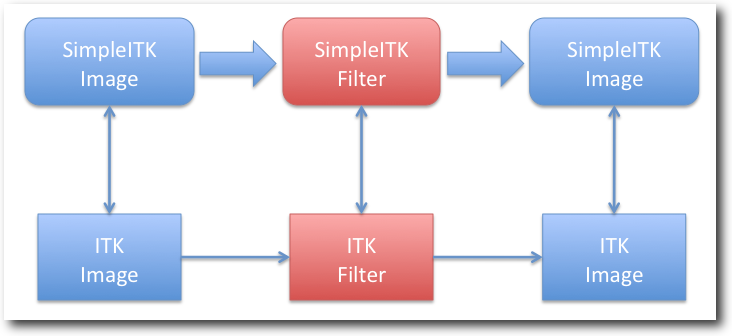
\includegraphics[width=.8\textwidth]{Images/FilterOverview_shadow}
\end{center}
\begin{itemize}
  \item SimpleITK filters create ITK filters
  \item Templated based on input type
  \item Output type is usually the same as input type
  \item Instantiated for many possible image types
\end{itemize}
\end{frame}

\begin{frame}[fragile]
\frametitle{Image and Filter Types}
\begin{columns}
  \begin{column}{0.5\textwidth}
    \begin{itemize}
      \item Dimensions
      \begin{itemize}
        \item 2 dimensional
        \item 3 dimensional
      \end{itemize}
      \item Scalar types
      \begin{itemize}
        \item $int8\_t$
        \item $uint8\_t$
        \item $int16\_t$
        \item $uint16\_t$
        \item $int32\_t$
        \item $uint32\_t$
        \item $float$
        \item $double$
        \item $std::complex< float >$
        \item $std::complex< double >$
      \end{itemize}
    \end{itemize}
  \end{column}

  \begin{column}{0.5\textwidth}
     \begin{itemize}
       \item Vector Types
       \begin{itemize}
         \item $int8\_t$
         \item $uint8\_t$
         \item $int16\_t$
         \item $uint16\_t$
         \item $float$
         \item $double$
       \end{itemize}
       \item Label Types
       \begin{itemize}
         \item $uint8\_t$
         \item $uint16\_t$
         \item $uint32\_t$
       \end{itemize}
    \end{itemize}
  \end{column}
\end{columns}
\end{frame}

\begin{frame}[fragile]
\frametitle{Filter Anatomy}
\begin{center}
  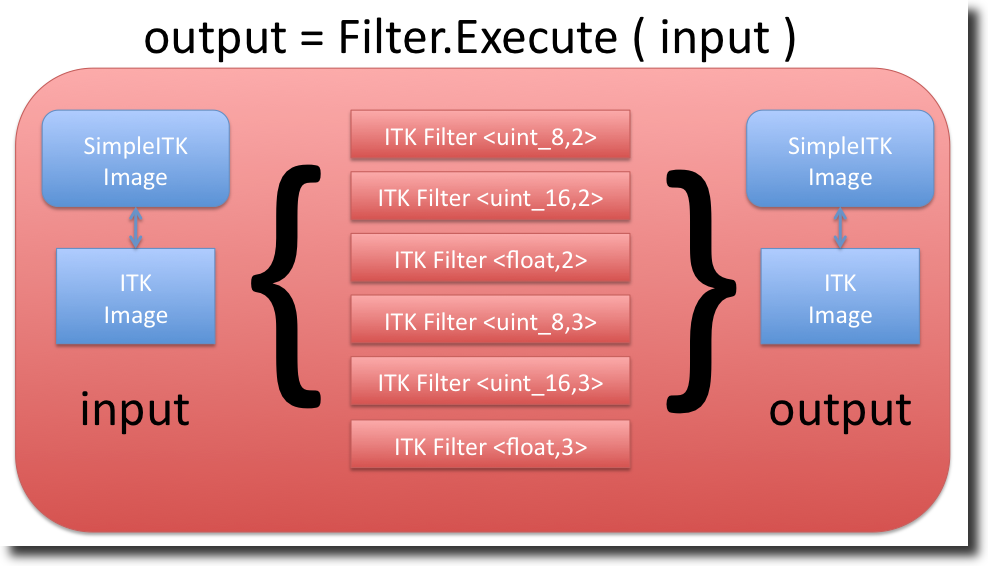
\includegraphics[width=.8\textwidth]{Images/FilterInternals_shadow}
\end{center}
\begin{itemize}
  \item Filter interrogates $input$
  \item Instantiates proper ITK filter
  \item Executes ITK filter
  \item Constructs $output$ from ITK image
\end{itemize}
\end{frame}

\subsection{Using Filters}
\begin{frame}{Using Filters}
\fontsize{36pt}{36pt}\selectfont
\center
\begin{center}
Using Filters
\end{center}
\end{frame}

\begin{frame}[fragile]
\frametitle{Object Paradigm (C++)}
\lstcpp
\begin{lstlisting}
#include <SimpleITK.h>
namespace sitk = itk::simple;
...
// Create a smoothing filter
sitk::SmoothingRecursiveGaussianImageFilter gaussian;

// Set a parameter
gaussian.SetSigma ( 2.0 );

// "Execute" the Filter
sitk::Image blurredImage = gaussian.Execute ( image );
\end{lstlisting}
\end{frame}

\begin{frame}[fragile]
\frametitle{Object Paradigm (C++)}
Flexibility
\lstcpp
\begin{lstlisting}
#include <SimpleITK.h>
namespace sitk = itk::simple;
...
// Create a smoothing filter
sitk::SmoothingRecursiveGaussianImageFilter gaussian;

// Set parameter(s), then execute
sitk::Image blurredImage = gaussian
                             .SetSigma ( 2.0 )
                             .Execute ( image );
\end{lstlisting}
\end{frame}

\begin{frame}[fragile]
\frametitle{Object Paradigm (C++)}
\lstcpp
\begin{lstlisting}
#include <SimpleITK.h>
namespace sitk = itk::simple;
...
blurredImage = sitk::SmoothingRecursiveGaussianImageFilter()
                         .SetSigma ( 2.0 )
                         .SetRadius ( 5 )
                         .Execute ( image );
\end{lstlisting}
One line: create anonymous filter, set parameters, and execute
\end{frame}

\begin{frame}[fragile]
\frametitle{``Function'' Paradigm (C++)}
\lstcpp
\begin{lstlisting}
#include <SimpleITK.h>
namespace sitk = itk::simple;
...
// Call the function version
// NB: Drop the "ImageFilter"!
// Signature:
/*
    sitk::Image SmoothingRecursiveGaussian (
            const Image&,
            double inSigma = 1.0,
            bool inNormalizeAcrossScale = false );
*/
sitk::Image blurredImage = sitk::SmoothingRecursiveGaussian (
                              image,
                              2.0,
                              false );
\end{lstlisting}
\end{frame}

\begin{frame}[fragile]
\frametitle{Mix \& Match (C++)}
\lstcpp
\begin{lstlisting}
#include <SimpleITK.h>
namespace sitk = itk::simple;
...
// Get our gaussian ready
sitk::SmoothingRecursiveGaussianImageFilter gaussian;
gaussian.SetSigma ( 2.0 );

// What is the effect on the image
sitk::Image difference = sitk::Subtract (
                           image,
                           gaussian.Execute ( image )
                           );
sitk::Image difference2 = sitk::Subtract (
                     image,
                     sitk::SmoothingRecursiveGaussian (
                       image, 2.0
                       )
                     );

\end{lstlisting}
\end{frame}



\subsection{Code Philosophy}
\begin{frame}{Code Philosophy}
\fontsize{36pt}{36pt}\selectfont
\center
\begin{center}
Code Philosophy
\end{center}
\end{frame}

\begin{frame}[fragile]
\frametitle{Filter Class Overview (C++)}
\lstcpp
\begin{lstlisting}
class SmoothingRecursiveGaussianImageFilter : (* \label{Declaration} *)
    public ImageFilter {
  typedef SmoothingRecursiveGaussianImageFilter Self; (* \label{Self} *)

  /** Default Constructor that takes no arguments
      and initializes default parameters */
  SmoothingRecursiveGaussianImageFilter(); (* \label{Constructor} *)

\end{lstlisting}
\begin{itemize}
  \item In line \ref{Declaration}, we declare a subclass of ImageFilter
  \item Line \ref{Self} creates a special typedef for use later
  \item The default constructor is line \ref{Constructor} (never any parameters)
\end{itemize}
\end{frame}


\begin{frame}[fragile]
\frametitle{Filter Class Overview (C++) Continued}
\lstcpp
\begin{lstlisting}
  /** Define the pixels types supported by this filter */
  typedef BasicPixelIDTypeList  PixelIDTypeList; (* \label{PixelIDTypeList} *)

\end{lstlisting}
\begin{itemize}
  \item Notice $PixelIDTypeList$ in line \ref{PixelIDTypeList}
  \item Used to instantiate ITK filters
  \item Determines valid input image types
  \item $BasicPixelIDTypeList$ expands to:
  \begin{itemize}
    \item $int8\_t$, $uint8\_t$
    \item $int16\_t$, $uint16\_t$
    \item $int32\_t$, $uint32\_t$
    \item $float$, $double$
  \end{itemize}
\end{itemize}
\end{frame}


\begin{frame}[fragile]
\frametitle{Filter Class Overview (C++) Continued}
\lstcpp
\begin{lstlisting}
  Self& SetSigma ( double t ) { ... return *this; }
  double GetSigma() { return this->m_Sigma; }

  Self& SetNormalizeAcrossScale ( bool t ) { ... }
  Self& NormalizeAcrossScaleOn() { ... }
  Self& NormalizeAcrossScaleOff() { ... }

  bool GetNormalizeAcrossScale() { ... }
\end{lstlisting}
\begin{itemize}
  \item Get/Set parameters
  \item Set methods always return $Self\&$ (more later)
  \item Generally, a direct mapping to ITK
  \item Boolean parameters generate $On$ and $Off$ methods
\end{itemize}
\end{frame}


\begin{frame}[fragile]
\frametitle{Filter Class Overview (C++) Continued}
\lstcpp
\begin{lstlisting}
  /** Name of this class */
  std::string GetName() const { ... }

  /** Print ourselves out */
  std::string ToString() const;
\end{lstlisting}
\begin{itemize}
  \item Return the name and description of the filter
\end{itemize}
\end{frame}


\begin{frame}[fragile]
\frametitle{Filter Class Overview (C++) Continued}
\lstcpp
\begin{lstlisting}
  /** Execute the filter on the input image */
  Image Execute ( const Image & );

  /** Execute the filter with parameters */
  Image Execute ( const Image &,
    double inSigma,
    bool inNormalizeAcrossScale );
};  /* End of class SmoothingRecursiveGaussian */

Image SmoothingRecursiveGaussian ( const Image& , (* \label{Function} *)
  double inSigma = 1.0,
  bool inNormalizeAcrossScale = false );

\end{lstlisting}
\begin{itemize}
  \item Run the filter on an image and return the result
  \item Notice extra function (line \ref{Function}), adds flexibility
  \item Drop $ImageFilter$ from class name to get function name
\end{itemize}

\end{frame}

\begin{frame}{Questions?}
\fontsize{36pt}{36pt}\selectfont
\center
\begin{center}
Questions?
\end{center}
\end{frame}


\subsection{Interface with ITK}
\begin{frame}[fragile]
\frametitle{Using ITK with SimpleITK}
Problem: Use ITK from SimpleITK (or vice versa)

\texttt{./ToITK input.nii output.nii}

Steps:
\begin{itemize}
\item Load image using SimpleITK
\item Filter using ITK
\item Save using OpenCV
\end{itemize}
\end{frame}

\begin{frame}[fragile]
\frametitle{To ITK}
Starting code: \texttt{ToITK/ToITK.cxx}\\
Directory: \texttt{SimpleITK-MICCAI-2011-Tutorial/Examples/AdvancedTutorial}
\begin{lstlisting}
namespace sitk = itk::simple;
...
  // Load the image via SimpleITK
  sitk::Image sitkImage = sitk::ReadImage ( inputFilename );

  // Construct the ITK Pipeline
  // Link pipeline to SimpleITK
  // Update pipeline
  // Create output SimpleITK image
  // Save image via SimpleITK
  sitk::WriteImage ( sOutput, outputFilename );
  return EXIT_SUCCESS;
\end{lstlisting}
\end{frame}

\begin{frame}[fragile]
\frametitle{ToITK -- Step 1: Construct the ITK Pipeline}
\begin{lstlisting}
  // Construct the ITK Pipeline
  typedef itk::Image<float,3> ImageType;
  typedef itk::MirrorPadImageFilter<ImageType,ImageType> PadFilterType;
  PadFilterType::SizeType upperBound, lowerBound;

  PadFilterType::Pointer pad = PadFilterType::New();
  for ( unsigned int i = 0; i < 3; i++ )
    {
      upperBound[i] = sitkImage.GetSize()[i];
      lowerBound[i] = sitkImage.GetSize()[i];
    }
  pad->SetPadUpperBound ( upperBound );
  pad->SetPadLowerBound ( lowerBound );
\end{lstlisting}
\end{frame}

\begin{frame}[fragile]
\frametitle{ToITK -- Step 2: Link pipeline to SimpleITK}
\begin{lstlisting}
  // Link pipeline to SimpleITK
  ImageType::Pointer inputImage = (ImageType*) sitkImage.GetImageBase();
  pad->SetInput ( inputImage );
\end{lstlisting}
\end{frame}

\begin{frame}[fragile]
\frametitle{ToITK -- Step 3: Update ITK Pipeline}
\begin{lstlisting}
  // Update pipeline
  pad->Update();
\end{lstlisting}
\end{frame}

\begin{frame}[fragile]
\frametitle{ToITK -- Step 4: Create the SimpleITK output image}
\begin{lstlisting}
  // Create output SimpleITK image
  sitk::Image sOutput ( pad->GetOutput() );
\end{lstlisting}
\end{frame}

\begin{frame}[fragile]
\frametitle{ToITK -- (Optional) Step 5: Show}
\begin{lstlisting}
  // (Optional) Show the results
  sitk::Show ( sOutput );
\end{lstlisting}
\end{frame}

\begin{frame}[fragile]
\frametitle{To ITK Solution}
\texttt{\textasciitilde/Source/AdvancedTutorial-build/ToITK/ToITKSolution \textbackslash\\
  \textasciitilde/Source/SimpleITK/Testing/Data/Input/RA-Float.nrrd \textbackslash\\
  /tmp/foo.nii}
\begin{center}
  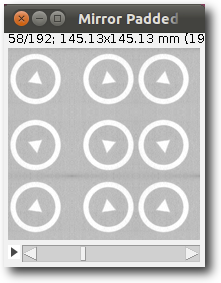
\includegraphics[width=0.3\textwidth]{Images/ToITKSolution_shadow}
\end{center}
\end{frame}


\subsection{Interface with OpenCV}
\begin{frame}[fragile]
\frametitle{To OpenCV}
Problem: Use SimpleITK from another image processing library (OpenCV)

\texttt{./ToOpenCV input.png output.png}

Steps:
\begin{itemize}
\item Load image using SimpleITK
\item Convert to OpenCV
\item Filter using OpenCV
\item Save using OpenCV
\end{itemize}
\end{frame}


\begin{frame}[fragile]
\frametitle{ToOpenCV}
Starting code: \texttt{ToOpenCV/ToOpenCV.cxx}\\
Directory: \texttt{SimpleITK-MICCAI-2011-Tutorial/Examples/AdvancedTutorial}
\begin{lstlisting}
#include <SimpleITK.h>
#include <opencv2/opencv.hpp>
namespace sitk = itk::simple;
...
  sitk::Image sitkImage = sitk::ReadImage ( inputFilename );

  // Convert SimpleITK to OpenCV image
  cv::Mat ocvImage;

  // Filter and write using OpenCV
  cv::Mat output;
  cv::medianBlur ( ocvImage, output, 5 );

  cv::imwrite ( outputFilename, output );
...
\end{lstlisting}
\end{frame}

\begin{frame}[fragile]
\frametitle{ToOpenCV -- Step 1}
Convert the SimpleITK image to a float
\begin{lstlisting}
  if ( sitkImage.GetPixelIDValue() != sitk::sitkFloat32 )
    {
    std::cout << "Input image is " << sitkImage.GetPixelIDTypeAsString()
              << " converting to float" << std::endl;
    sitkImage = sitk::Cast ( sitkImage, sitk::sitkFloat32 );
    }
\end{lstlisting}
\end{frame}

\begin{frame}[fragile]
\frametitle{ToOpenCV -- Step 2}
Get SimpleITK pixel data
\begin{lstlisting}
  // Convert SimpleITK to OpenCV image
  cv::Mat ocvImage ( sitkImage.GetHeight(), sitkImage.GetWidth(), CV_32F,
                     (void*)sitkImage.GetBufferAsFloat() );
\end{lstlisting}
\end{frame}

\begin{frame}[fragile]
\frametitle{ToOpenCV -- Step 3 (Optional)}
Display the before and after
\lstcppa
\begin{lstlisting}
// NB: the imshow function requires 8-bit data, so convert
cv::Mat temp;
ocvImage.convertTo ( temp, CV_8U );
cv::imshow ( "original slice", temp );
output.convertTo ( temp, CV_8U );
cv::imshow ( "bilateral filtering", temp );

std::cout << "Press any key to continue" << std::endl;
cv::waitKey();
\end{lstlisting}
\end{frame}

\begin{frame}[fragile]
\frametitle{To OpenCV Solution}
\texttt{\textasciitilde/Source/AdvancedTutorial-build/ToOpenCV/ToOpenCV \textbackslash \\
  \textasciitilde/Source/SimpleITK/Testing/Data/Input/cthead1.png \textbackslash \\
/tmp/head.png}
\begin{center}
  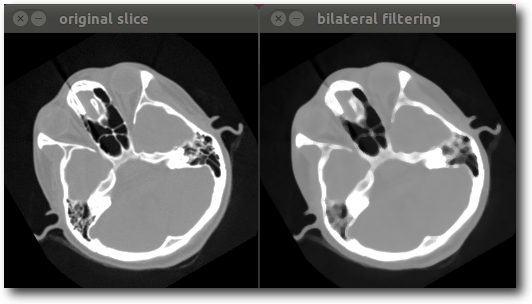
\includegraphics[width=0.5\textwidth]{Images/ToOpenCVSolution_shadow}
\end{center}
\end{frame}


\begin{frame}[fragile]
\frametitle{To OpenCV and Back}
Problem: Use OpenCV to process a SimpleITK volume slice-by-slice

\texttt{./ToOpenCVAndBack input.nii output.nii}

Steps:
\begin{itemize}
\item Load image using SimpleITK
\item Extract slice
\item Convert to OpenCV
\item Filter using OpenCV
\item Past slice back to SimpleITK
\item Save result
\end{itemize}
\end{frame}


\begin{frame}[fragile]
\frametitle{To OpenCV and Back}
Starting code: \texttt{ToOpenCVAndBack/ToOpenCVAndBack.cxx}\\
Directory: \texttt{SimpleITK-MICCAI-2011-Tutorial/Examples/AdvancedTutorial}
\begin{lstlisting}
namespace sitk = itk::simple;
...
sitk::Image sitkImage = sitk::ReadImage ( inputFilename );

for ( unsigned int s = 0; s < sitkImage.GetDepth(); s++ )
  {
  // Extract a slice
  // Go through ITK to grab the data
  // Convert ITK to OpenCV image
  // Filter using OpenCV
  // Convert back to SimpleITK
  // Paste the image back into SimpleITK
  }
sitk::WriteImage ( sOutput, outputFilename );
\end{lstlisting}
\end{frame}

\begin{frame}[fragile]
\frametitle{To OpenCV and Back - Step 1: Extract a slice}
\begin{lstlisting}
// Extract a slice
std::vector<unsigned int> size = sitkImage.GetSize();
size[2] = 1;
std::vector<int> index ( 3, 0 );
index[2] = s;
std::cout << "Extracting: " << s << std::endl;
sitk::Image slice = sitk::RegionOfInterest ( sitkImage, size, index );

if ( slice.GetPixelIDValue() != sitk::sitkFloat32 )
  {
  slice = sitk::Cast ( slice, sitk::sitkFloat32 );
  }
\end{lstlisting}
\end{frame}

\begin{frame}[fragile]
\frametitle{To OpenCV and Back - Step 2: Convert to OpenCV}
\begin{lstlisting}
// Convert ITK to OpenCV image
  cv::Mat ocvImage ( slice.GetHeight(), slice.GetWidth(),
                     CV_32F, (void*)sitkImage.GetBufferAsFloat() );
\end{lstlisting}
\end{frame}

\begin{frame}[fragile]
\frametitle{To OpenCV and Back - Step 3: Filter using OpenCV}
\begin{lstlisting}
  // Filter using OpenCV
  cv::Mat output;
  cv::Sobel ( ocvImage, output, -1, 1, 1 );
\end{lstlisting}
\end{frame}

\begin{frame}[fragile]
\frametitle{To OpenCV and Back - Step 4: Back to SimpleITK}
\begin{lstlisting}
  // Convert back to SimpleITK
  sitk::ImportImageFilter importer;
  importer.SetSize ( size );
  importer.SetSpacing ( sitkImage.GetSpacing() );
  importer.SetOrigin ( sitkImage.GetOrigin() );
  importer.SetBufferAsFloat ( output.ptr<float>() );

  sitk::Image toSimpleITKImage = importer.Execute();
\end{lstlisting}
\end{frame}

\begin{frame}[fragile]
\frametitle{To OpenCV and Back - Step 5: Paste back into SimpleITK volume}
\begin{lstlisting}
  // Paste the image back into SimpleITK
  // Paste ( Destination, Source, SourceSize, SourceIndex, DestIndex )
  sOutput = sitk::Paste ( sOutput, toSimpleITKImage,
            toSimpleITKImage.GetSize(), std::vector<int> ( 3,0 ), index );
\end{lstlisting}
\end{frame}

\begin{frame}[fragile]
\frametitle{To OpenCV and Back -- (Optional) Step 6: Show}
\begin{lstlisting}
  // (Optional) Show the results
  sitk::Show ( sOutput );
\end{lstlisting}
\end{frame}

\begin{frame}[fragile]
\frametitle{To OpenCV and Back Solution}
\texttt{\textasciitilde/Source/AdvancedTutorial-build/\textbackslash\\
ToOpenCVAndBack/ToOpenCVAndBack \textbackslash \\
  \textasciitilde/Source/SimpleITK/Testing/Data/Input/RA-Float.nrrd \textbackslash \\
  /tmp/foo.nii}
\begin{center}
  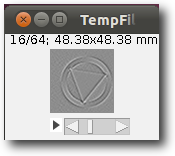
\includegraphics[width=0.4\textwidth]{Images/ToOpenCVAndBackSolution_shadow}
\end{center}
\end{frame}


\subsection{Java -- Groovy}

\begin{frame}{Java/Groovy}
\fontsize{36pt}{36pt}\selectfont
\center
\begin{center}
Using SimpleITK from Java/Groovy
\end{center}
\vspace{20pt}
\begin{center}
\fontsize{11pt}{11pt}\selectfont
\texttt{Examples/AdvancedTutorial/Java/Example.groovy}
\end{center}
\end{frame}

\begin{frame}{Groovy}
\begin{itemize}
  \item Language build on Java
  \item Superset of Java
  \item Can be used interactively
\end{itemize}
\end{frame}

\begin{frame}[fragile]
\frametitle{Groovy}
\lstjava
\begin{lstlisting}
import org.itk.simple.*;

Image i;
i = new Image ( 64, 64, 64, PixelIDValueEnum.sitkInt16 );
SimpleITK.show ( i, "Blank" );
\end{lstlisting}
\fontsize{8pt}{8pt}\selectfont
\texttt{groovysh -classpath
 ./SimpleITK-Build/SimpleITK-Build/Wrapping/org.itk.simple.jar}
\end{frame}

% Too advanced?
%% \begin{frame}
%% \frametitle{Extending SimpleITK}
%% JSON and friends
%% \end{frame}
